% !Mode:: "TeX:UTF-8"
\title{实验二 HDFS基础入门 实验报告}
\author{江昱峰 21009200038} 
\documentclass {article}
\usepackage[UTF8]{ctex}
\usepackage{graphicx}
\usepackage{float}
\usepackage{hyperref}
\usepackage{makecell}
\usepackage{listings}
\begin{document}
	%\begin{sloppypar}
	\maketitle{}
	\section{背景介绍}
		之前通过Hadoop伪分布式集群搭建,已经将我们的基础环境配置完成。我们在此基础上,将HDFS分布式文件系统作为Hadooop的文件存储系统,结合自身高容错、高吞吐以及可扩展的特点,为我们大数据的大数据集存储提供保障。
	
	\section{实验目的}
		实践并掌握HDFS基础,具体包括以下两部分内容:
		\begin{itemize}
			\item HDFS的shell命令——增删改查;
			\item HDFS的shell管理命令。
		\end{itemize}
	
	\section{实验知识}	
		HDFS概论:Hadoop分布式文件系统(HDFS)是指被设计成适合运行在通用硬件(commodity hardware)上的分布式文件系统(Distributed File System)。它和现有的分布式文件系统有很多共同点。但同时,它和其他的分布式文件系统的区别也是很明显的。HDFS是一个高度容错性的系统,适合部署在廉价的机器上。HDFS能提供高吞吐量的数据访问,非常适合大规模数据集上的应用。HDFS放宽了一部分POSIX约束,来实现流式读取文件系统数据的目的。HDFS在最开始是作为Apache Nutch搜索引擎项目的基础架构而开发的。HDFS是Apache Hadoop Core项目的一部分。
	
	\section{实验要求}
		完成HDFS基础,具体包括以下两部分任务:
		\begin{itemize}
			\item HDFS的shell命令——增删改查;
			\item HDFS的shell管理命令。
		\end{itemize}
	
	\section{实验环境}
		本次实验实验环境为青椒课堂平台的Linux(Centos 7.5)操作系统。
	
	\section{实验步骤与结果分析}
		\subsection{HDFS的shell命令——增删改查}
			\subsubsection{任务1:操作HDFS文件或目录}
				shell命令实操:
				\begin{enumerate}
					\item 查看HDFS根目录下结构。
					\begin{figure}[H]
						\centering
						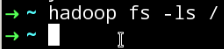
\includegraphics{figures/fig1.png}
					\end{figure}
				
					因为我们根目录下没有问价或文件夹,因此不显示内容。
					\item 在HDFS根目录下创建root文件夹。
					\begin{figure}[H]
						\centering
						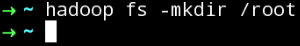
\includegraphics{figures/fig2.png}
					\end{figure}
				
					\item 在本地/root目录下创建hadoop.txt文件,添加如下内容:\\
					hadoop hdfs yarn \\
					hello hadoop
					\begin{figure}[H]
						\centering
						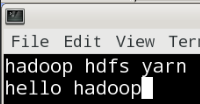
\includegraphics{figures/fig3.png}
					\end{figure}
					
					\item 将本地hadoop.txt上传到HDFS目录/root/下。
					\begin{figure}[H]
						\centering
						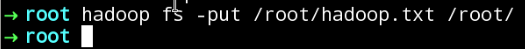
\includegraphics{figures/fig4.png}
					\end{figure}
				
					\item 将HDFS目录文件/root/hadoop.txt复制到根目录下并查看内容。
					\item 删除HDFS目录文件/root/hadoop.txt。
					\begin{figure}[H]
						\centering
						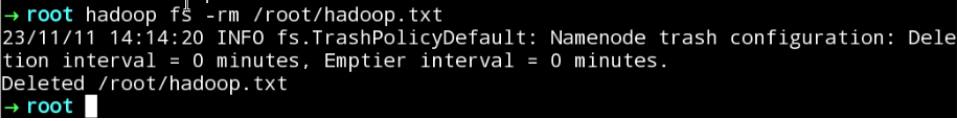
\includegraphics[width=4.5in]{figures/fig5.jpg}
					\end{figure}
				
					\item 将HDFS目录文件/hadoop.txt迁移到HDFS目录/root/下并查看迁移是否成功。
					\begin{figure}[H]
						\centering
						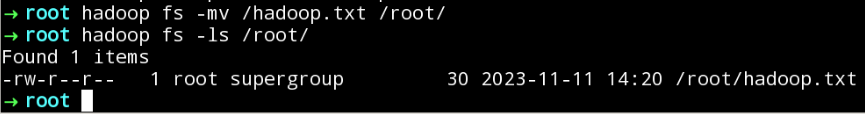
\includegraphics[width=4.5in]{figures/fig6.png}
					\end{figure}
				
					\item 将HDFS目录文件/root/hadoop.txt复制到本地根目录下并查看。
					\begin{figure}[H]
						\centering
						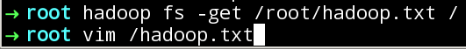
\includegraphics{figures/fig7.png}
					\end{figure}
					\begin{figure}[H]
						\centering
						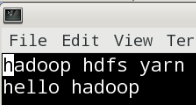
\includegraphics{figures/fig8.png}
					\end{figure}
				\end{enumerate}
			
			\subsubsection{任务2:查看、追加、合并文本}
				appendToFile命令实操:
				\begin{enumerate}
					\item 在本地当前目录(/headless)下创建a.txt,b.txt,c.txt文件。
					\begin{figure}[H]
						\centering
						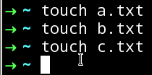
\includegraphics{figures/fig9.png}
					\end{figure}
				
					\item 分别添加内容123,456,789。
					\begin{figure}[H]
						\centering
						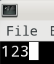
\includegraphics{figures/fig10.png}
					\end{figure}
					\begin{figure}[H]
						\centering
						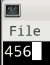
\includegraphics{figures/fig11.png}
					\end{figure}
					\begin{figure}[H]
						\centering
						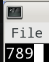
\includegraphics{figures/fig12.png}
					\end{figure}
				
					\item 在HDFS根目录下创建abc.txt文件并查看。
					\begin{figure}[H]
						\centering
						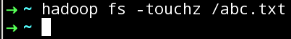
\includegraphics{figures/fig13.png}
					\end{figure}
				
					\item 将本地a.txt,b.txt,c.txt追加到abc.txt文件。
					\begin{figure}[H]
						\centering
						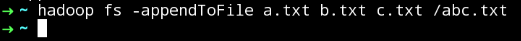
\includegraphics{figures/fig14.png}
					\end{figure}
				
					\item 查看abc.txt文件。
					\begin{figure}[H]
						\centering
						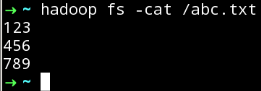
\includegraphics{figures/fig15.png}
					\end{figure}
				\end{enumerate}
			
			 	getmerge命令实操:
			 	\begin{enumerate}
			 		\item 将刚才创建的a.txt,b.txt,c.txt文件上传到HDFS根目录。
			 		\begin{figure}[H]
			 			\centering
			 			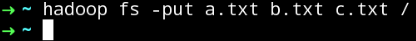
\includegraphics{figures/fig16.png}
			 		\end{figure}
		 		
		 			\item 将HDFS根目录下*.txt文件下载到本地/root/sum.txt。
		 			\begin{figure}[H]
		 				\centering
		 				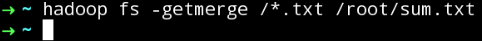
\includegraphics{figures/fig17.png}
		 			\end{figure}
			 	\end{enumerate}
		 	
	 	\subsection{HDFS的shell管理命令}
	 		\subsubsection{任务1:任务一:修改权限命令}
	 			修改权限命令实操:
	 			\begin{enumerate}
	 				\item 在本地当前目录创建测试文件a.txt并添加内容如下:\\
	 				Centos7 \\
	 				JDK1.8 \\
	 				Hadoop2.7.7
	 				\begin{figure}[H]
	 					\centering
	 					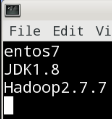
\includegraphics{figures/fig18.png}
	 				\end{figure}
 				
 					\item 将文件上传到HDFS根目录。
 					\begin{figure}[H]
 						\centering
 						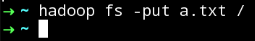
\includegraphics{figures/fig19.png}
 					\end{figure}
					
					\item 修改a.txt文件权限为所有用户可读不可写可执行并进行查看。
					\begin{figure}[H]
						\centering
						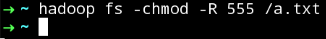
\includegraphics{figures/fig20.png}
					\end{figure}
				
					\item 修改a.txt文件所属用户和用户组为root并查看。
					\begin{figure}[H]
						\centering
						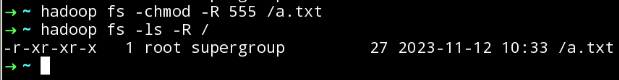
\includegraphics[width=4.5in]{figures/fig21.png}
					\end{figure}
					\begin{figure}[H]
						\centering
						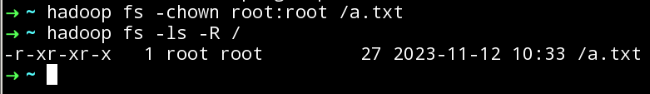
\includegraphics[width=4.5in]{figures/fig22.png}
					\end{figure}
	 			\end{enumerate}
	 			
	 		\subsubsection{任务2:任务二:统计、设置副本命令}
	 			统计命令实操:
	 			\begin{enumerate}
	 				\item 统计根目录下目录数,文件数和字节数。
	 				
	 				(1)创建HDFS目录/tmp。
	 				\begin{figure}[H]
	 					\centering
	 					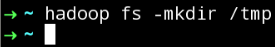
\includegraphics{figures/fig23.png}
	 				\end{figure}
	 				
	 				(2)将上节任务a.txt移动到HDFS目录/tmp下。
	 				\begin{figure}[H]
	 					\centering
	 					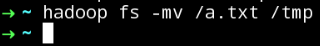
\includegraphics{figures/fig24.png}
	 				\end{figure}
 				
 					\item 统计文件系统的容量、可用空间和已用空间信息。
 					\begin{figure}[H]
 						\centering
 						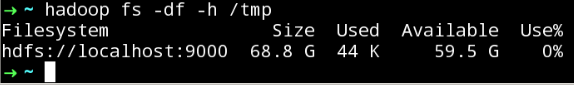
\includegraphics[width=4.5in]{figures/fig25.png}
 					\end{figure}
 				
 					\item 统计/tmp目录下所有文件和文件夹的大小。
 					\begin{figure}[H]
 						\centering
 						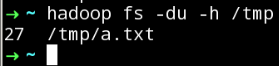
\includegraphics{figures/fig26.png}
 					\end{figure}
	 			\end{enumerate}
			
				设置副本命令实操:
				
				设a.txt副本数为2。
				\begin{figure}[H]
					\centering
					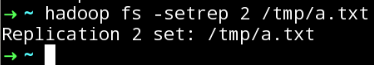
\includegraphics{figures/fig27.png}
				\end{figure}
	
	\section{结果分析}
		HDFS中的Shell操作管理命令与一般的Linux、Windows操作系统的命令相类似,只是在前面加上了"hadoop fs -"。
			
	\section{困难解决}
		本次实验较为简单,没有遇到困难。
	
	\section{心得体会}
		做完本次实验,除了掌握了实验目的部分中所有内容的收获之外,我还有以下几点心得体会:
		\begin{itemize}
			\item 实践并掌握了HDFS查看、追加、合并文本,修改权限命令,统计、设置副本命令等内容;
			\item 对比分析了HDFS与一般Linux系统中Shell命令的异同点。
		\end{itemize}
	
%\end{sloppypar}
\end{document}
\endinput